\newcommand{\h}[1]{\textit{#1}}
\newcommand{\bp}{BasePhyLayer}
\newcommand{\bm}{BaseMacLayer}


\section{modelling}

\emph{Note: }We denote a Layer in a general meaning by 'physical layer' 
or 'MAC layer' and our concrete C++ classes by \h{\bp} or \h{\bm}.


\subsection{overview}

Here we present the design- and interface details of the OMNeT-module 
\h{\bp} to meet the requirement specification. That includes:

\begin{enumerate}
 \item internal class diagram of \h{\bp} and relation to \h{\bm}
 \item interface description for all involved C++ classes
 \item flow charts for reception of MacPacket from upper layer and 
 AirFrame from the channel
 \item some detailed flow charts for important sub processes
\end{enumerate}


\subsection{classgraph}

We start with the classgraph for the OMNeT-module \h{\bp} that shows 
its C++ classes, relations to other OMNeT-modules (especially \h{\bm})
and the OMNeT-messages sent between them.

The \h{\bp} holds a list\req{analogueMulti} of AnalogueModels and a pointer to a Decider. Thus the AnalogueModel and the Decider are submodules of \h{\bp}. This way one is able to change\req{analogueExtensible}\req{deciderExtensible} and replace\req{analogueIndependent}\req{deciderIndependent} them independently from the \h{\bp}.

\begin{figure}[H]
 \centering
 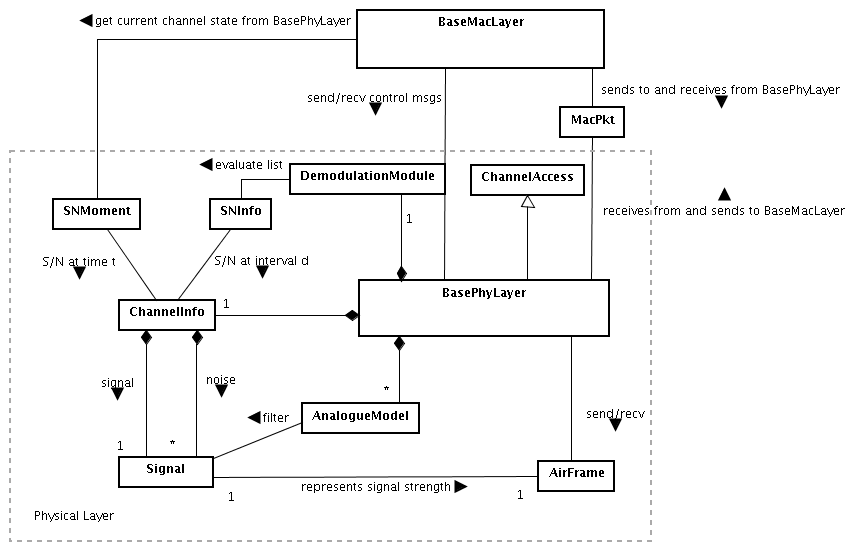
\includegraphics[width = \textwidth]{modelling/class_diagram.png}
 \caption{class graph}
 \label{fig: classgraph}
\end{figure}


\subsection{The \h{\bp} interface}

In this section we focus on how one is able to communicate with the 
\h{\bp}, i.e. especially the \h{\bm} which is connected to the \h{\bp}
in three ways:

\begin{enumerate}
 \item OMNeT-channel for data messages
 \item OMNeT-channel for control messages
 \item a reference to \h{\bp}.
\end{enumerate} 

The data channel is used to send and receive\req{packetFromMac} MacPkts to and from the \h{\bp}.

The control channel is used by the \h{\bp} to inform the \h{\bm} about
certain events\req{provactive}, like the TX\_OVER\req{txover} message 
which indicates the end of a sending transmission.

The reference provides a passive way\req{provpassive} for the  \h{\bm} to  get information about the current channel state\req{channelstate} and to get\req{currentmode} and set\req{switchmode} the current state (RX, TX, SLEEP).
Switching times\req{switchtimes} from one radio state to another are controlled internaly by a state machine. \saf{mode state machine}.


\begin{figure}[H]
 \centering
 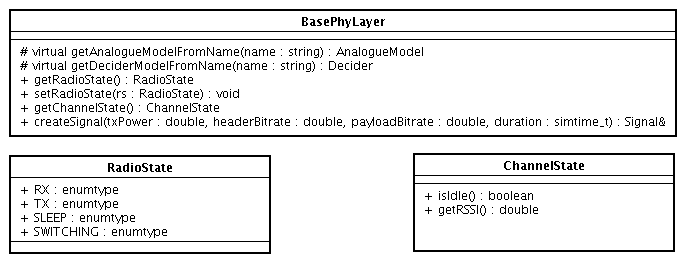
\includegraphics[width = \textwidth]{modelling/BasePhyLayer_members.png}
 \caption{BasePhyLayer interface}
 \label{fig: BasePhyLayer interface}
\end{figure}



\subsection{AnalogueModel and Signal}
\label{AM and Signal}

%The Signal is designed one-dimensional (power-over-time) by default with a specified time point for start and end of the Signal. The owner is able
%to add and request values at a specific time point\req{sendInfoTXPower}.
%The Method getTimeIterator() returns an appropriate SignalTimeIterator needed for applying AnalogueModels to the Signal.

%\begin{quote}
%\emph{NOTE: Anyone who subclasses Signal should make shure to have a properly
%working SignalTimeIterator (subclassed) for it. The SignalTimeIterator should always iterate over every time stamp in each dimension. This way simple AnalogueModels will be able to filter the Signal independent from its dimension.}
%\end{quote}

%Further the Signal is set the packets bitrate over time\req{sendInfoBitrate},  the Move of the Host\req{sendInfoMove}, the size of the packet\req{sendInfoSize} and the channel dimensions\req{sendInfoChannel} by \h{\bp}.
%
%\emph{See also \ref{AirFrame and Signal}.}
 
\begin{figure}[H]
 \centering
 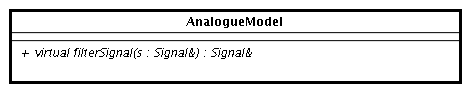
\includegraphics[width = \textwidth]{modelling/AnalogueModel_members.png}
 \caption{analogue model interface}
 \label{fig: analogue model interface}
\end{figure}
%
%The AnalogueModel offers functionality to filter a referenced signal\req{analogueFilter} in a specified interval\req{rcvFilterSignals} (e.g. preamble\req{rcvFilterPreamble}) or at a single point in time.

%Three basic AnalogueModel classes are foreseen to be plugged into Phy-Layer to simulate pathloss\req{analogueSimPathloss}, shadowing\req{analogueSimShadowing} and fading\req{analogueSimFading}.\\
%\h{\bp} is designed to apply an arbitrary number of AnalogueModels to a Signal.

\begin{figure}[H]
 \centering
 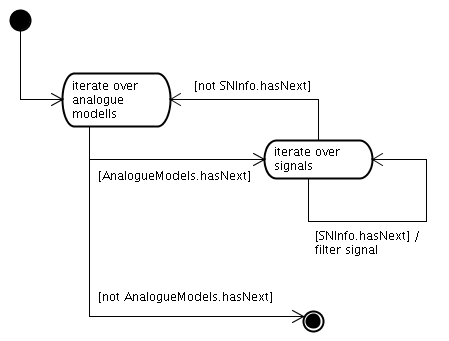
\includegraphics[width = 0.8\textwidth]{modelling/apply_analogue_modells_detail.png}%[width=300pt]
 \caption{application of analogue models}
 \label{fig: application analogue models}
\end{figure}



\subsection{SNInfo and ChannelInfo}

ChannelInfo keeps track of all AirFrames on the channel. It does not differentiate between \textit{signal} and \textit{noise}. \h{\bp} is able to
add and remove references to certain AirFrames to and from ChannelInfo.\\
ChannelInfo is able to record the whole channel over time from a start to a stop signal and can return a vector of Signals (references) that intersect with a given time interval.\\
SNInfo is created by \h{\bp} when a packet arrives to collect all signals from the channel that intersect with the reception time interval of the packet.

\begin{figure}[H]
 \centering
 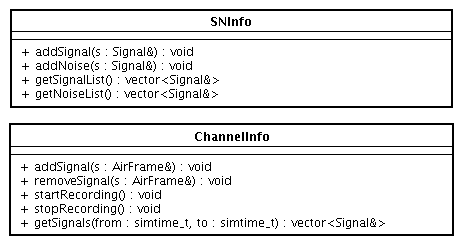
\includegraphics[width = \textwidth]{modelling/ChannelInfo_members.png}
 \caption{channel details}
 \label{fig: channel details}
\end{figure}




\subsection{Decider}

The Decider has two tasks:
\begin{enumerate}
	\item It decides whether we are able to receive a certain packet by evaluting
	the SNInfo for the packets preamble time interval, otherwise the packet will 	be considered noise\req{rcvClassify}
	\item When a packet has been received and is not noise the Decider 	returns a DeciderResult for that packet, that only contains if the packet was received correct or not correct by default\req{rcvIsCorrect}.
\end{enumerate}

A Decider that gives a richer DeciderResult (e.g. bitwise errors\req{deciderBitwise}) must be subclassed and implemented by the user.

\begin{figure}[H]
 \centering
 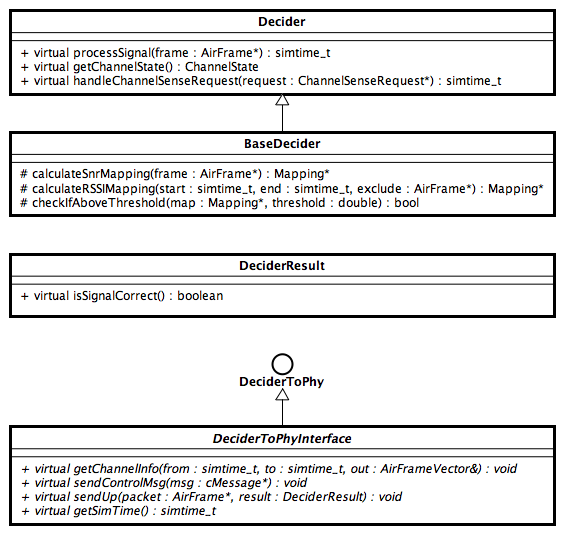
\includegraphics[width = \textwidth]{modelling/DeciderModule_members.png}
 \caption{Decider interface}
 \label{fig: Decider interface}
\end{figure}


\subsection{AirFrame}
\label{AirFrame and Signal}

AirFrame and Signal are both constructed by \h{\bp} with the help of MacToPhyControlInfo.
It is shown below how nessecary information for sending/receiving is distributed. Signal is already discussed in \ref{AM and Signal}.

\h{\bp} calculates duration\req{sendInfoDuration} and preamble duration\req{sendInfoPreambleDuration} of the packet and adds it to the AirFrame. 
To be able to control the sending process\req{sendControl} of another AirFrame every AirFrame has a unique id and a specific type which secifies if this is a normal AirFrame or a control-AirFrame.


\begin{figure}[H]
 \centering
 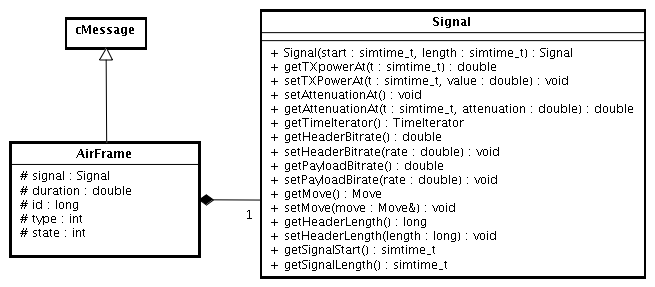
\includegraphics[width = \textwidth]{modelling/AirFrame_members.png}
 \caption{member arrangement in AirFrame and Signal}
 \label{fig: member AirFrame}
\end{figure}



\subsection{receiving a MacPkt}

On reception of a MacPkt from the MAC layer, \h{\bp} checks if:
\begin{enumerate}
	\item the radio is in TX state\req{sendPreqMode},
	\item it is not already sending a packet\req{sendPreqSending} and
	%\item the channel is idle\req{sendPreqIdle} (this is no hard requirement, \h{\bp} could send anyway).
\end{enumerate} 

If one of conditions is not fulfilled it will throw an error.\\

The MacToPhyControlInfo object attached to the MacPkt contains the information needed by \h{\bp} when constructing Signal and AirFrame to send to the channel. Right now it contains:

\begin{enumerate}
	\item the channel for sending\req{sendCtrlChannel},
	\item header bitrate\req{sendCtrlHeaderBitrate},
	\item payload bitrate\req{sendCtrlBitrate},
	\item TX Power\req{sendCtrlTXPower} and
	\item the size of the packet\req{sendCtrlSize}.

\end{enumerate}


\begin{figure}[H]
 \centering
 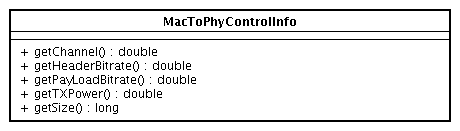
\includegraphics[width = \textwidth]{modelling/MacToPhyCtrlInfo_members.png}
 \caption{MacToPhyControlInfo interface}
 \label{fig: MacToPhyCtrlInfo interface}
\end{figure}

\h{\bp} is responsilbe for creating AirFrame and Signal and attaching information (parameters) to them. For detailed arrangement of information in Signal and AirFrame see \ref{AirFrame and Signal}.
When the AirFrame is complete and sent, \h{\bp} schedules a TX\_OVER message to the \h{\bm}(via control-message).

\begin{figure}[H]
 \centering
 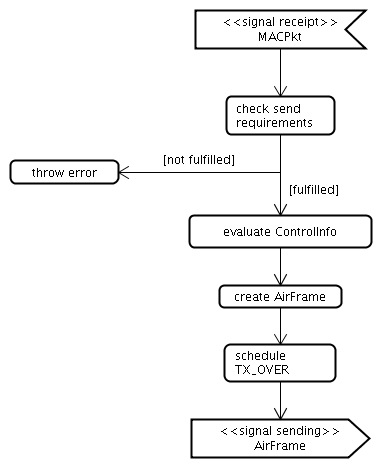
\includegraphics[width = 0.8\textwidth]{modelling/onMACPkt.png}
 \caption{sending process}
 \label{fig: sending process}
\end{figure}





\subsection{Receiving and processing an AirFrame}

The reception of an AirFrame is divided into:
\begin{enumerate}
	
	\item optional propagation delay\req{rcvSimDelay},
	\item reception of the preamble\req{rcvSimPreamble},
	\item application of AnalogueModels to the corresponding SNInfo\req{rcvSimAttenuation},
	\item decision whether packet is considered noise (Decider),
	\item reception of the packet\req{rcvSimDuration}.
\end{enumerate}

Afterwards the packet is either dropped (if considered noise) or processed. 

\begin{figure}[H]
 \centering
 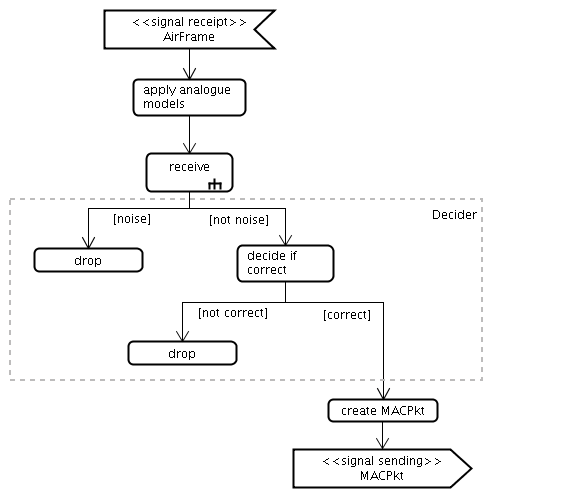
\includegraphics[width = 0.8\textwidth]{modelling/onAirFrame.png}
 \caption{receiving process}
 \label{fig: receiving process}
\end{figure}

The receiving process is modelled internally by a state machine that schedules the AirFrame that is received (since we have a pointer to it from the beginning) everytime a delay/time interval shall be simulated. That saves us the creation of additional self-messages.


\begin{figure}[H]
 \centering
 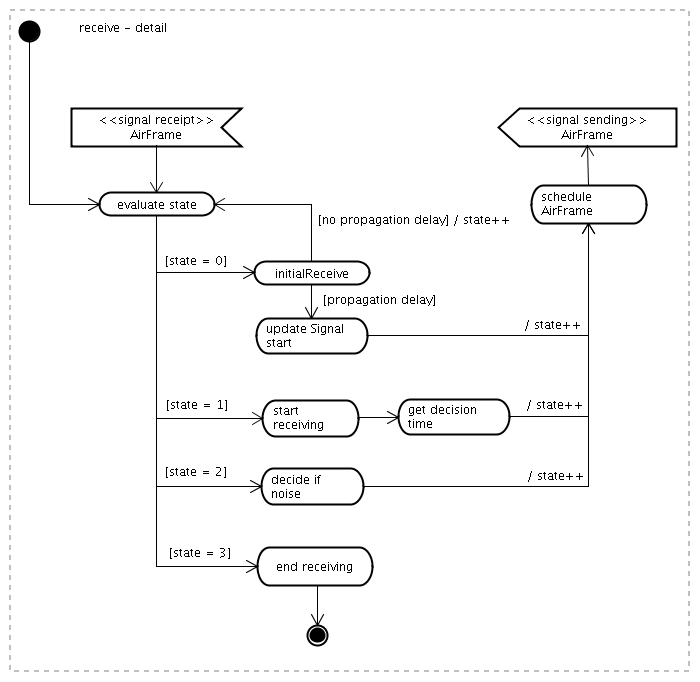
\includegraphics[width = \textwidth]{modelling/receive_detail.png}
 \caption{receive detail}
 \label{fig: receive detail}
\end{figure}

%When the preamble of a packet is completely received, \h{\bp} constructs a SNInfo for the preamble, applies the AnalogueModels to it and passes it to the Decider to find out whether this packet is considered noise.

%\begin{figure}[H]
% \centering
% 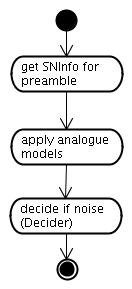
\includegraphics[width = 0.2\textwidth]{modelling/end_preamble_detail.png}
% \caption{end preamble detail}
% \label{fig: end preamble detail}
%\end{figure}

%In case a received packet is not \textit{noise} it is processed, i.e. \h{\bp} creates the corresponding SNInfo for the packet, applies AnalogueModels to it and passes the result to the Decider to check whether the packet was received correctly. If so, a MacPkt is created and handed up to Phy-Layer\req{rcvPassToMAC}.


\subsection{the .ned-file}

The .ned-file of the \h{\bp} has the following parameters:

\begin{itemize}
\item usePropagationDelay as \textit{boolean}\req{confDelay}
\item analogueModels as \textit{XML}\req{confAnalogue}\req{confAnalogueParam}
\item decider as \textit{XML}\req{confDecider}\req{confDeciderParam}
\item thermalNoise as \textit{numeric const}\req{confNoise}
\item sensitivity as \textit{numeric const}\req{confSens}
\item maximal TX power as \textit{numeric const}\req{confMaxTXPower}
\item switchTimeRX as \textit{numeric const}\req{confSwitchingTimes}
\item switchTimeTX as \textit{numeric const}\req{confSwitchingTimes}
\item switchTimeSleep as as \textit{numeric const}\req{confSwitchingTimes}
\end{itemize}

The parameters "analogueModels" and "decider" holds which AnalogueModels and Decider to be used together with their parameters in XML format. The exact format still has to be declared!

%\subsection{provide status information to MAC}

%Passively provided information\req{provpassive}: \h{\bm} is equipped with a reference to \h{\bp} in order to obtain information
%about channelstate\req{channelstate} and current radio state\req{currentmode} by
%simple method calls. \\
%Actively provided information\req{provactive}: A cMessage of the kind TX\_OVER
%is sent to MAC layer when a sending transmission is over\req{txover}, \saf{sending process}.



%\subsection{send packets}

%Since \h{\bm} has a reference to \h{\bp} it can obtain information about the state the radio is is currently in\req{sendPreqMode}, it is not already sending to the channel on its own\req{sendPreqSending} and the channel is idle\req{sendPreqIdle} via method calls, \saf{BasePhyLayer interface}.

%The class MacToPhyControlInfo is designed as the container for control info\req{packetFromMac} the MAC layer
%wants to attach to the packet given down to Phy-Layer for sending.
%The packet itself is handed down as a MacPkt via OMNeT-channel. 















